\documentclass[12pt]{article}
	\usepackage{geometry}
	\geometry{margin=1in}
	\usepackage[utf8]{inputenc}
	\usepackage{graphicx}
	\usepackage{amsmath}
	\usepackage{mathrsfs}
	\usepackage{amssymb}
	\usepackage[backend=bibtex,style=numeric]{biblatex}
	\usepackage{algorithm}
	\usepackage{algpseudocode}
	\usepackage{hyperref}

	\addbibresource{bibliografia.bib}
	
	\title
		{
		\vspace{-30mm}\begin{figure}[h]
		\centering
		
\includegraphics[width=2in]{./Include/logo_polimi.png}
		\end{figure}
		Anderson Acceleration for Fixed-Point Iterations
		}
		
	\author{Martino Ischia\\ \footnotesize{Supervisor: Prof. Formaggia}}
	\date{January 2021}
		
		
	\begin{document}
		\maketitle
		\begin{abstract}
			\noindent The goal of this project is twofold.\\
			Firstly, develop a C++ interface for accelerating a converging sequence of vectors.
			It should be at the same time open for extensions, in case the user wants to implement its own algorithm,
			and efficient in the solution of large systems.\\
			Secondly, making use of said interface to implement Anderson acceleration strategy and apply it on ...\\
			The reader not interested in the C++ implementation can safely skip section \ref{sec:C++}.
		\end{abstract}
		\tableofcontents
		\pagebreak
		
		
		\section{Introduction}
			A fixed-point problem consists in finding the point (a vector in $\mathbb{R}^n$) that satisfies the
			following:
			\begin{equation}
			x = g(x)
			\label{eq:g}
			\end{equation}
			where g is a function from $\mathbb{R}^n$ to $\mathbb{R}^n$.\\
			It is clearly equivalent to the problem of finding the roots of a generic function,
			that is often tackled by employing Newton-Raphson iterative algorithm.
			In many concrete applications, though, the cost of computing the Jacobian of a function
			is not practical, not to mention that there might be issues in starting the
			iterations from a proper guess.\\
			Considering the fixed-point form and solving through fixed-point iterations has also some limitations, the main one being
			a slow convergence: in fact most of the times the convergence is linear.\\
			Several strategies have been described in the literature to improve the speed
			of convergence of a vector sequence: we could refer to them as acceleration methods.
			This project focuses on one of them,
			proposed by \citeauthor{Anderson} \cite{Anderson} in \citeyear{Anderson}.
			
			\subsection{Anderson Algorithm}
				There are many equivalent ways to formulate Anderson acceleration method.
				I report the one in \citeauthor{Walker} \cite{Walker}.\\
				Several adjustment can be made to address specific problems, but in this
				project only this simple form is considered. The interested reader can
				refer to \cite{Fang} \cite{Walker}.
				
			\begin{algorithm}
				\caption{Anderson algorithm}
				\label{alg1}
			\begin{algorithmic}
				\State Given $x_0$ and $m \geq 1$
				\State Set $x_1 = g(x_0)$
				\For {$k = 1, 2, ...$ until convergence}
				\State Set $m_k = min\{m, k\}$
				\State Set $F_k = (f_{k-m_k}, ... , f_k)$, where $f_i = g(x_i)-x_{i}$
				\State Determine $\alpha^{(k)} = (\alpha^{(k)}_0 , ..., \alpha^{(k)}_{m_k} )^T$, subject to 
				$\sum^{m_k}_{i=0} {\alpha_i = 1}$, that solves
				
				\begin{equation}
				\min_{\alpha=(\alpha_0,...,\alpha_{m_k} )^T} \|F_k \alpha\|_2
				\end{equation}
				
				\State Set $x_{k+1} = (1-\beta) \sum^{m_k}_{i=0} {\alpha_i^{(k)} x_{k-m_{k}+i}}	+\beta \sum^{m_k}_{i=0} {\alpha_i^{(k)} g(x_{k-m_{k}+i})}$   
				\EndFor
				\end{algorithmic}	
				\end{algorithm}
				
			The new value is obtained through a linear combination of the previous iterates and their evaluations.
			The coefficients are found through a minimization problem, in this case written as a constrained
			problem, but an unconstrained form is usually chosen for the implementation \cite{Fang}\cite{Walker}.
			
			A compact way to write the update formula, albeit not fully rigorous, is as follows:
			\begin{equation}
				\label{eq:2}
				x_{k+1}=x_{k} + \beta f_k -(\mathscr{X}_k + \beta \mathscr{F}_k)(\mathscr{F}_k^T \mathscr{F}_k)^{-1}\mathscr{F}_k^T f_k
			\end{equation}
			where \begin{itemize}
			\item	$\mathscr{X}_k=[\Delta x_{k-m}...\Delta x_{k-1}]$ with $\Delta x_{i}=x_{i+1}-x_i$  
			\item $\mathscr{F}_k=[\Delta f_{k-m}...\Delta f_{k-1}]$ with $\Delta f_{i}=f_{i+1}-f_i$ and $f_i$ is still $g(x_i)-x_{i}$
			\end{itemize}
			Notice that the algorithm depends on two parameters: $\beta$, a relaxation parameter which has also
			a special interpretation when the algorithm is seen as a multisecant method \cite{Fang}, and $m$,
			a memory parameter, which represents the number of previous iterates considered in the calculations.
			
					
		\section{C++ interface for fixed-point problems}
		\label{sec:C++}
		
		\subsection{Overview}

		The code can be found at \href{https://github.com/martinoischia/Anderson-acceleration}{this link} and is subdivided into two directories:
		\verb|Include| and \verb|src|.\\
		The \verb|Include| directory contains (mostly) external utilities that
		are used.\\
		The \verb|source| directory contains the interface and the implementation of the classes, as well as
		examples of increasing level of complexity.\\
		The only library needed for compiling the code is the header-only \href{http://eigen.tuxfamily.org/}{Eigen}
		version 3 (I am using 3.3). The path of the Eigen library has to be specified in \verb|/src/Makefile|.\\
		Special care has been put into documenting the code with the use of the \verb|Doxygen| package 
		(\verb|graphviz| package is also required in order to produce cool looking graphs). The interested reader
		is suggested to consult the documentation by running \verb|make doc| in the \verb|src| directory.
		An \verb|html| directory will be generated, containing an \verb|index.html| file. Open it in a web browser for consulting the documentation.
		
		In the next sections I will describe the most interesting features of the code, so again I redirect to the documentation the reader
		who wants a complete picture of the functionalities provided by the inteface.\\
		The code is based on two classes: \verb|Iterator|,
		a functor that provides the next value of a sequence, and
		\verb|FixedPointIterator|, which composes the former and
		provides a \verb|compute| method for producing iterations until some criteria are satisfied.
		
		
		\subsection{Traits}
		The classes mentioned above, \verb|Iterator| and \verb|FixedPointIterator|, are generic in the sense that
		they do not define the types they use: they inherit them from an external struct.
		The code offers two options, \verb|DenseTraits| and \verb|SparseTraits|, but user can define his own.\\
		From eq. \ref{eq:g} it is clear that a fixed-point problem needs a type for vector $x$ and a type for iteration function $g$.
		Moreover, since Anderson algorithm requires calculations on matrices, a matrix type is needed.
		The matrix type is in fact what differentiates \verb|DenseTraits| from \verb|SparseTraits|,
		with obvious meaning.\\
		For the definition of this types, we rely on the Eigen library, a fast and versatile
		C++ template library for linear algebra. 
		
		This Traits structs are used by other classes by mean of inheritance: the \verb|Traits| macro
		is defined in \verb|Accelerators.hpp| as, for example, \verb|SparseTraits|, and all classes inherit
		from \verb|Traits|, obtaining in such a way a definition of \verb|Vector|, \verb|IterationFunction| and \verb|Matrix| types
		as well as some utilities related to this types.
		
		
		\subsection{The Iterator family}
		The first ingredient is a class that stores the fixed-point iteration function in eq. \ref{eq:g} and provides the next value
		of a vector sequence. The \verb|Iterator| class overloads the call
		operator to provide such new value. In this base class, what the call operator does is rather trivial:
		it just calls the iteration function applied to the last value stored in the argument.\\
		To be more precise, the operator has the signature
		\begin{verbatim}
			Traits::Vector Iterator::operator()(const std::deque<Vector>& past)
		\end{verbatim}
		It is intuitive that the \verb|past| parameter represents an object storing the past vectors assumed by a certain sequence.
		The choice for the data structure to be an \verb|std::deque| will be clear when we will describe the \verb|FixedPointIterator| class.
		
		Concerning the constructor, the use of the so-called universal reference in combination with \verb|std::forward|
		allows to move the argument when possible (an \verb|std::function|, which is the type of the iteration function,
		may potentially have a big size in the form of a function object).
		
		The \verb|Iterator| class is the base class for more advanced classes which try to speed-up the convergence
		process.
		In fig. \ref{fig:1} is shown the inheritance diagram of the \verb|Iterator| class.
		\begin{figure}
			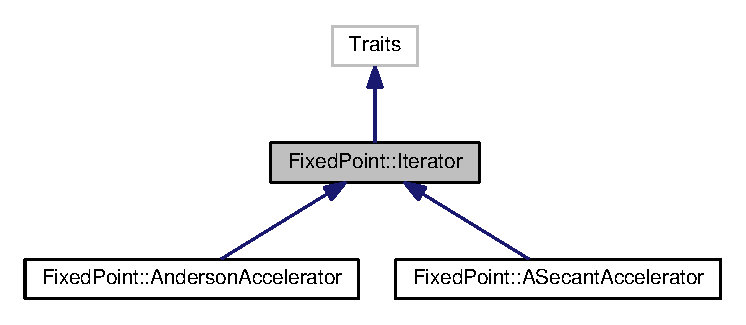
\includegraphics{./Include/inheritance.eps}
			\centering
			\caption{Inheritance diagram for the \texttt{Iterator} class}
			\label{fig:1}
		\end{figure}
		In addition to the \verb|AndersonAccelerator| class, another class called \verb|ASecantAccelerator| is provided,
		wihch is a simpler version of Anderson in which the memory parameter has value two.\\
		The derived classes make use of polymorphism to overload the function call operator.\\
		Let us dive deeper into the implementation of Anderson algorithm.
		
		
		\subsection {Implementation of Anderson algorithm}
		Equation \ref{eq:2} shows that to compute the next value of the sequence two matrices are needed:
		$\mathscr{X}_k$ and $\mathscr{F}_k$.\\
		If the \verb|Iterator| class is called all of a sudden
		to compute the next value of a sequence given as input, the \verb|SetUp| method must be called to compute $\mathscr{X}_k$ and $\mathscr{F}_k$ up
		to the values involving the last iteration (the function call operator takes care of the last part).
		But most of the times Anderson iterations want to be kept running until convergence: for this reason we
		store two matrices \verb|X| and \verb|F| which are updated only in the last column at each call of the call operator.\\
		These two matrices have a special type to perform the update operation easily: it is the \verb|RotatingMatrix|
		template class. The template argument is chosen to provide the most efficient insert strategy, the one in which
		the new inserted column replaces the oldest column when the maximum size of the matrix has been reached.
		
		Concerning the update formula \ref{eq:2}, the term $\mathscr{F}_k^T \mathscr{F}_k^{-1}\mathscr{F}_k^T f_k$
		represents the solution of a least square problem. It is well known that solving this so-called normal
		equations is a bad choice from the numerical point of view, due to ill-conditioning of the matrices.
		For this reason, the least square problem is solved by mean of the QR decomposition of the matrix $\mathscr{F}_k$. In particular the
		Householder rank-revealing QR decomposition with column-pivoting is used, that is a good compromise
		between numerical stability and efficiency.\\
		Interestingly enough, the result of the update formula \ref{eq:2} is independent of the ordering of the columns
		of $\mathscr{X}_k$ and $\mathscr{F}_k$. This is important since it 
		the proper reordering of the columns of the \verb|RotatingMatrix| class would add another computational cost.\\		
		This fact can be seen from the QR decomposition but is more easily seen from the normal equations.\\
		Calling $P$ a generic permutation matrix (which has the property
		that $P^T=P^{-1}$), swapping column of a matrix $A$ is achieved by performing the matrix multiplication $AP$.
		Substituting $\mathscr{X}_k$ and $\mathscr{F}_k$ with their permuted counterpart, eq. \ref{eq:2} becomes
		\begin{equation}
			x_{k+1}=x_{k} + \beta f_k -(\mathscr{X}_k + \beta \mathscr{F}_k)P(P^T \mathscr{F}_k^T \mathscr{F}_k P)^{-1}P^T \mathscr{F}_k^T f_k
		\end{equation}
		Thus, for properties of the inverse of a matrix
		\begin{equation}
			x_{k+1}=x_{k} + \beta f_k -(\mathscr{X}_k + \beta \mathscr{F}_k)P P^T (\mathscr{F}_k^T \mathscr{F}_k)^{-1} P P^T \mathscr{F}_k^T f_k
		\end{equation}
		By simplifying $P P^T$ one gets that the solution is invariant with respect to exchanging columns of $\mathscr{X}_k$ and $\mathscr{F}_k$.
		
		One last note: \citeauthor{Walker} \cite{Walker} make use of factor-updating QR decomposition, which is a more efficient algorithm
		for computing the QR factors of $\mathscr{F}_k$ from the ones of $\mathscr{F}_{k-1}$. We did not consider it in this project
		because such algorithm was not available in the Eigen library. Moreover the rank-1 updated QR decomposition would not work
		when the oldest column of the matrix gets replaced.
		
		
		\subsection {The \texttt{FixedPointIterator} class}
		The \texttt{FixedPointIterator} class governs the solving of the fixed-point problem.\\
		It has the following private attributes:
		\begin{itemize}
		\item \verb|iterator|, an \verb|std::unique_ptr| to an \verb|Iterator| object that produces the iterates. The unique pointer
		allows to compose an object in the polymorphic \verb|Iterator| family, for example an \verb|AndersonAccelerator| object
		\item \verb|options|, an options struct, controlling maximum iterations, tolerances and printing styles
		\item \verb|history|, an \verb|std::deque<Vector>| containing the history of the vector sequence. The choice of the
		data structure is due to the fact that, when the number of vectors reaches the threshold of \verb|options::memory|, the last stored
		vector is eliminated from the front and the new vector is added to the back. This operation is more suited for an
		\verb|std::deque| rather than an \verb|std::vector|.
		\item \verb|iteration|, an integer representing the number of executed iterations by the \verb|compute| method.
		\end{itemize}
		
		Concerning the public member functions, the class  provides two \verb|compute| methods, one with no parameters and the second one
		with an initial vector as a starting guess. These methods make use of the \verb|history| member to compute iterations until
		convergence. In fact, the initial guess is used only in the case \verb|history| is empty. If \verb|history| is empty
		and no guess is provided, a default vector of zeros is used.\\
		The \verb|printResult| method is one of the possibility to output a result.
		
		
		\subsection{A first example}
			The file \verb|main_simple_problem.cpp| constitutes a first working example of the previously defined classes.\\
			It solves a simple nonlinear problem in 3D, taken from book \cite{Quarteroni}, whose fixed-point form converges to
			the solution $(0,1/3,0)$.\\
			All the parameters of interest are read from an input file, exploiting GetPot, a simple but effective utility.
			This allows to not recompile the code when we want to test a different parameter.
			
			\begin{figure}
			{\scriptsize
			% GNUPLOT: LaTeX picture with Postscript
\begingroup
  % Encoding inside the plot.  In the header of your document, this encoding
  % should to defined, e.g., by using
  % \usepackage[cp1252,<other encodings>]{inputenc}
  \inputencoding{cp1252}%
  \makeatletter
  \providecommand\color[2][]{%
    \GenericError{(gnuplot) \space\space\space\@spaces}{%
      Package color not loaded in conjunction with
      terminal option `colourtext'%
    }{See the gnuplot documentation for explanation.%
    }{Either use 'blacktext' in gnuplot or load the package
      color.sty in LaTeX.}%
    \renewcommand\color[2][]{}%
  }%
  \providecommand\includegraphics[2][]{%
    \GenericError{(gnuplot) \space\space\space\@spaces}{%
      Package graphicx or graphics not loaded%
    }{See the gnuplot documentation for explanation.%
    }{The gnuplot epslatex terminal needs graphicx.sty or graphics.sty.}%
    \renewcommand\includegraphics[2][]{}%
  }%
  \providecommand\rotatebox[2]{#2}%
  \@ifundefined{ifGPcolor}{%
    \newif\ifGPcolor
    \GPcolorfalse
  }{}%
  \@ifundefined{ifGPblacktext}{%
    \newif\ifGPblacktext
    \GPblacktexttrue
  }{}%
  % define a \g@addto@macro without @ in the name:
  \let\gplgaddtomacro\g@addto@macro
  % define empty templates for all commands taking text:
  \gdef\gplbacktext{}%
  \gdef\gplfronttext{}%
  \makeatother
  \ifGPblacktext
    % no textcolor at all
    \def\colorrgb#1{}%
    \def\colorgray#1{}%
  \else
    % gray or color?
    \ifGPcolor
      \def\colorrgb#1{\color[rgb]{#1}}%
      \def\colorgray#1{\color[gray]{#1}}%
      \expandafter\def\csname LTw\endcsname{\color{white}}%
      \expandafter\def\csname LTb\endcsname{\color{black}}%
      \expandafter\def\csname LTa\endcsname{\color{black}}%
      \expandafter\def\csname LT0\endcsname{\color[rgb]{1,0,0}}%
      \expandafter\def\csname LT1\endcsname{\color[rgb]{0,1,0}}%
      \expandafter\def\csname LT2\endcsname{\color[rgb]{0,0,1}}%
      \expandafter\def\csname LT3\endcsname{\color[rgb]{1,0,1}}%
      \expandafter\def\csname LT4\endcsname{\color[rgb]{0,1,1}}%
      \expandafter\def\csname LT5\endcsname{\color[rgb]{1,1,0}}%
      \expandafter\def\csname LT6\endcsname{\color[rgb]{0,0,0}}%
      \expandafter\def\csname LT7\endcsname{\color[rgb]{1,0.3,0}}%
      \expandafter\def\csname LT8\endcsname{\color[rgb]{0.5,0.5,0.5}}%
    \else
      % gray
      \def\colorrgb#1{\color{black}}%
      \def\colorgray#1{\color[gray]{#1}}%
      \expandafter\def\csname LTw\endcsname{\color{white}}%
      \expandafter\def\csname LTb\endcsname{\color{black}}%
      \expandafter\def\csname LTa\endcsname{\color{black}}%
      \expandafter\def\csname LT0\endcsname{\color{black}}%
      \expandafter\def\csname LT1\endcsname{\color{black}}%
      \expandafter\def\csname LT2\endcsname{\color{black}}%
      \expandafter\def\csname LT3\endcsname{\color{black}}%
      \expandafter\def\csname LT4\endcsname{\color{black}}%
      \expandafter\def\csname LT5\endcsname{\color{black}}%
      \expandafter\def\csname LT6\endcsname{\color{black}}%
      \expandafter\def\csname LT7\endcsname{\color{black}}%
      \expandafter\def\csname LT8\endcsname{\color{black}}%
    \fi
  \fi
    \setlength{\unitlength}{0.0500bp}%
    \ifx\gptboxheight\undefined%
      \newlength{\gptboxheight}%
      \newlength{\gptboxwidth}%
      \newsavebox{\gptboxtext}%
    \fi%
    \setlength{\fboxrule}{0.5pt}%
    \setlength{\fboxsep}{1pt}%
\begin{picture}(5668.00,2834.00)%
    \gplgaddtomacro\gplbacktext{%
      \csname LTb\endcsname%%
      \put(1220,806){\makebox(0,0)[r]{\strut{}$1\times10^{-10}$}}%
      \put(1220,1138){\makebox(0,0)[r]{\strut{}$1\times10^{-8}$}}%
      \put(1220,1470){\makebox(0,0)[r]{\strut{}$1\times10^{-6}$}}%
      \put(1220,1803){\makebox(0,0)[r]{\strut{}$0.0001$}}%
      \put(1220,2135){\makebox(0,0)[r]{\strut{}$0.01$}}%
      \put(1220,2467){\makebox(0,0)[r]{\strut{}$1$}}%
      \put(1340,440){\makebox(0,0){\strut{}$0$}}%
      \put(2001,440){\makebox(0,0){\strut{}$5$}}%
      \put(2662,440){\makebox(0,0){\strut{}$10$}}%
      \put(3324,440){\makebox(0,0){\strut{}$15$}}%
      \put(3985,440){\makebox(0,0){\strut{}$20$}}%
      \put(4646,440){\makebox(0,0){\strut{}$25$}}%
      \put(5307,440){\makebox(0,0){\strut{}$30$}}%
    }%
    \gplgaddtomacro\gplfronttext{%
      \csname LTb\endcsname%%
      \put(190,1636){\rotatebox{-270}{\makebox(0,0){\strut{}Residual}}}%
      \put(3323,140){\makebox(0,0){\strut{}Iteration \#}}%
      \csname LTb\endcsname%%
      \put(4404,2470){\makebox(0,0)[r]{\strut{}Fixed-point iterations}}%
      \csname LTb\endcsname%%
      \put(4404,2270){\makebox(0,0)[r]{\strut{}Anderson algorithm}}%
    }%
    \gplbacktext
    \put(0,0){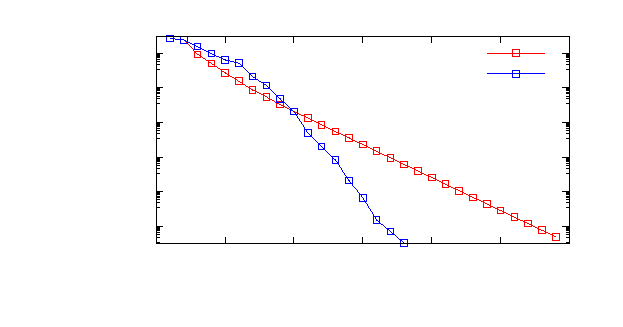
\includegraphics{./Include/simple_example_residuals}}%
    \gplfronttext
  \end{picture}%
\endgroup
}
			\centering
			\caption{Residual vs interation number for a simple 3D problem}
			\label{fig:simple}
			\end{figure}
			
			Figure \ref{fig:simple} shows the residual at each iteration when standard fixed-point iterations are used 
			and when Anderson algorithm is used with mixing parameter $\beta$ equal to $1$ and memory parameter $m$ equal to $5$.
			Fixed-point iterations converge in $28$ iterations whereas Anderson algorithm converges in $17$.

		\section{FEM application}
		\label{sec:FEM}
			aaa

		\pagebreak			
			\printbibliography[heading=bibintoc,
			title={Bibliography}]
						
					
	\end{document}
								